\documentclass[11pt]{article}
\usepackage[margin=1in]{geometry}
\usepackage{amsmath,amssymb,booktabs,graphicx,xcolor,listings}
\usepackage[hidelinks]{hyperref}
\usepackage{microtype}
\definecolor{guardgreen}{HTML}{047857}
\definecolor{codebackground}{HTML}{F3F6F8}
\lstset{basicstyle=\small\ttfamily,breaklines=true,columns=fullflexible,
  keepspaces=true,showstringspaces=false,backgroundcolor=\color{codebackground},
  frame=single,framerule=0pt,xleftmargin=5pt,xrightmargin=5pt,
  keywordstyle=\color{guardgreen}\bfseries}
\newcommand{\FullMedian}{0.527}
\newcommand{\FullLow}{0.409}
\newcommand{\FullHigh}{0.604}
\newcommand{\ParseMedian}{0.144}
\newcommand{\MarginalMedian}{0.401}
\newcommand{\FuzzDraws}{5000}
\newcommand{\FuzzUnique}{3434}
\newcommand{\FuzzRejects}{233}
\newcommand{\FuzzErrors}{194}
\newcommand{\FuzzUpperPercent}{0.0599}
\newcommand{\OriginalObservations}{2112}
\newcommand{\FullObservations}{384}
\newcommand{\EdgeObservations}{280}

\title{\texttt{sqlguardllm}: Policy-Driven Validation and Rewriting of LLM-Generated SQL\\[4pt]
  \large A Reproducible Systems Study}
\author{Juan Castillo\\\small\url{https://github.com/jmmana/sqlguardllm}}
\date{November 26, 2026\\\small Manuscript for author review; not submitted to arXiv}

\begin{document}
\maketitle
\begin{abstract}
SQL generated by a language model can be a valid read-only query while still
accessing another tenant's records or a restricted column. We describe
\texttt{sqlguardllm}, an open-source Python library that validates SQL syntax
trees against application-owned policies and regenerates queries with row
filters and result limits. Its engine is deterministic, model-independent,
and does not make network or model calls. We contribute an executable study
that distinguishes syntax-level admission from result-level policy compliance.
The study uses 48 authored query templates in two tenant contexts, executing
against SQLite, DuckDB, and PostgreSQL compiled to WebAssembly through PGlite.
For each runtime, an independently constructed database containing only
authorized rows provides the result oracle. Across 288 full-policy observations,
216 allowed-query results matched that oracle and 72 forbidden reads were
rejected, with no observed execution errors or over-rejections. An ablation
without row filters produced 59 result-policy mismatches per 96 observations.
Native PostgreSQL row policies and column grants matched the full guard on
the tested workload. Median warm validation times were 0.504--0.538 ms;
database execution is excluded. These are descriptive results on a small,
study-authored workload, not a proof of security or an estimate of performance
on unseen attacks. Raw decisions, timings, fixtures, source fingerprints,
and reproduction instructions accompany the manuscript.
\end{abstract}

\section{Introduction}
Natural-language database interfaces move part of query construction from
application code into a model. The resulting SQL is an untrusted program
submitted to a privileged data-access component. A successful prompt injection,
an ordinary model mistake, or a directly malicious caller may therefore have
the same consequence at the SQL boundary: a query that exceeds the caller's
authority. Prior work documents security failures in text-to-SQL systems
\cite{peng2024security} and the difficulty of detecting sensitive-data leakage
\cite{song2024securesql}. More recent evaluation work explicitly separates
query utility from compliance with role-based access policies
\cite{fei2026rbac}.

Read-only credentials address an important part of this problem, but do not
by themselves express which rows or columns a caller may read. Likewise,
the presence of \texttt{SELECT} says little about authorization. A query that
counts all invoices, reads a private email address, or joins records across
tenants may be read-only and executable while violating the application's
policy. Native database controls, including row-level security (RLS) and
column privileges, are established mechanisms for addressing these issues
\cite{postgresrls}. Application-layer validation can complement them by
providing a portable policy boundary, structured errors for agents, and
consistent query rewriting across supported parser dialects.

This paper presents the design and an initial execution-oriented evaluation
of \texttt{sqlguardllm}. The library builds on SQLGlot \cite{sqlglot}; we do not
claim a new SQL parser, a new access-control model, or the invention of
security-oriented query rewriting. The contributions are (i) a documented
composition of statement validation, object restrictions, per-occurrence
row-filter injection, and SQL regeneration behind a stable result contract;
(ii) a transparent, machine-readable execution workload and physically
restricted reference databases; and (iii) a measured ablation and a native
RLS comparison that expose the distinction between query shape and authorized
results. The study is a systems artifact with explicitly limited coverage.

\section{Threat Model and Policy Boundary}
The attacker controls the entire SQL string. The policy, authenticated caller
context, database credentials, and execution wrapper are trusted application
inputs. The guard does not authenticate users, interpret natural-language
intent, or determine whether the application's chosen policy is appropriate.
The caller must execute the returned SQL rather than the original string and
must treat a rejected result as non-executable.

A policy specifies allowed physical tables, hidden columns, row predicates
with trusted context placeholders, and a maximum result size. Optional
features include function allowlists, complexity limits, masking, aggregate
restrictions, and output-dialect translation. The execution study concentrates
on table/column restrictions and tenant filters; optional privacy and cost
features are not empirically established by its results.

Let $D$ be a database, $c$ an authenticated context, and $P$ a policy. For a
physical relation $R$, write $D_{P,c}(R)$ for the rows satisfying its policy
predicate, exposing only authorized columns. For an admitted query $Q$ and
rewrite $T$, the intended result-level property on the tested fragment is
\begin{equation}
 \operatorname{bag}\bigl(\operatorname{exec}(T(Q,P,c),D)\bigr)
 = \operatorname{bag}\bigl(\operatorname{cap}_{m}
       (\operatorname{exec}(Q,D_{P,c}))\bigr),
 \label{eq:oracle}
\end{equation}
where $m$ is the configured result cap. Queries whose syntax references a
forbidden object must be rejected even if execution would happen to return
an empty result. Equation~\ref{eq:oracle} describes the study's test oracle;
it is not a theorem proved for arbitrary SQL. Ordered test queries determine
which rows precede a cap, while the comparison preserves duplicate rows and
ignores output ordering.

The boundary does not cover inference from permitted aggregates, timing
channels, side effects in unlisted user-defined functions, arbitrary parser
differentials, or exhaustion of database resources. A row cap limits output,
not scan cost. Least-privilege credentials, native permissions where available,
timeouts, and policy review remain necessary deployment controls. Function
allowlisting is relevant when a database exposes user-defined functions;
the default denylist cannot characterize every possible function.

\section{System Design}
\subsection{Validation and the result contract}
An application compiles a \texttt{Policy} into a reusable \texttt{Guard}.
For each call, SQLGlot parses the input in the declared dialect. The guard
checks that the input contains one query statement and walks the tree to
reject writes, DDL, session-changing operations, and locking nodes, including
operations nested below a query root. It resolves physical table sources
across common-table expressions (CTEs) and subqueries, checks table and
column restrictions, and applies configured function and complexity rules.
Unparseable input and missing filter context cause rejection.

The \texttt{check()} method returns a \texttt{CheckResult} containing \texttt{ok},
the regenerated \texttt{sql} when admitted, referenced tables, applied
filters, and structured violations with codes and explanations.
\texttt{Guard.enforce()} returns the admitted SQL or raises an exception.
The library does not execute database statements. Its optional MCP server
adds an execution wrapper; the experiments call the library directly.
The separate \texttt{explain()} interface provides richer provenance for
application interfaces and audits. Explanations and rewritten SQL may contain
bound context values and require appropriate handling before being shared
with a model or another party.

\subsection{Filtering physical table occurrences}
Appending a tenant predicate to the outermost \texttt{WHERE} clause is
insufficient for arbitrary joins, subqueries, and Boolean expressions.
Instead, each occurrence of a filtered physical table becomes a derived
table, preserving its external alias. For tenant 7, the input
\begin{lstlisting}[language=SQL]
SELECT id, total FROM invoices
WHERE tenant_id = 999 OR 1 = 1
ORDER BY id
\end{lstlisting}
is regenerated in the demonstration policy as
\begin{lstlisting}[language=SQL]
SELECT id, total
FROM (
  SELECT * FROM invoices WHERE tenant_id = 7
) AS invoices
WHERE tenant_id = 999 OR 1 = 1
ORDER BY id LIMIT 100
\end{lstlisting}
The outer tautology still operates only over the restricted derived table.
The same transformation applies to aliases in self-joins and to occurrences
inside CTEs and scalar subqueries. Trusted context values are converted into
escaped SQL literals in the syntax tree; they are not obtained from model
output. This is AST literal binding, not database-driver parameter binding.
The policy templates themselves are trusted configuration.

\subsection{Restrictions and regeneration}
Hidden-column references are checked beyond projection lists, including
predicates and expressions in grouping and ordering clauses. Stars over
tables with hidden columns are conservatively rejected. Without complete
metadata, conservative resolution may reject otherwise legitimate ambiguous
queries; the workload does not measure that full ambiguity space.
After validation and row-filter injection, the guard adds or reduces the
outer result limit and generates SQL from the transformed tree. Executing
the regenerated string narrows the boundary between the parsed program and
the executed program, but does not eliminate dialect mismatches in general.

\section{Experimental Method}
\subsection{Workload and independent execution oracle}
The study-authored execution workload contains 24 benign templates, 12
tenant-isolation stress templates, and 12 forbidden-read templates. Each is
evaluated for tenants 1 and 2. Benign templates include harmless occurrences
of SQL keywords in strings and comments, joins, grouping, aggregates, CTEs,
correlated subqueries, a window function, unions, and an existing limit.
Isolation templates include tautologies, explicit requests for the other
tenant, self-joins, nested CTEs, unions, and aggregates over unrestricted
tables. Forbidden reads exercise private-column use in several clauses,
derived tables and CTEs, stars, and access to a disallowed table.

The synthetic fixture contains 12 invoices, 8 customers, 4 branches, and
one secret row across two tenants. Invoice amounts and identifiers differ
between tenants so that aggregate leakage is detectable without relying on
an output sentinel. For every runtime, the harness constructs three databases:
one complete database and one physically restricted database per tenant.
Reference databases contain only that tenant's rows, omit the private email
column, and omit the secret table. For an allowed query, its unmodified SQL
runs against the reference database. The candidate's result is compared with
that reference as a bag of positional row values, including multiplicity.
Thus the reference does not call the guard or reuse its rewrite algorithm.
The cap is eight rows; templates that can exceed it use explicit ordering.
An oracle execution error aborts the study rather than counting as a defense.

The 48 templates are distinct from the project's existing regression corpus,
but were authored as part of this study with knowledge of the implementation.
They are not an independent held-out benchmark or a representative sample of
production SQL. The two tenant contexts and repeated runtimes are correlated
observations, not additional independent attack families.

\subsection{Methods and outcome definitions}
We evaluate five configurations. The \emph{keyword filter} rejects a
case-insensitive list of write-related keywords anywhere in the text.
The \emph{read-only shape} configuration uses the library's statement and
function checks with a result cap but no table, column, or row policy.
The \emph{no-row-filters} ablation keeps table/column restrictions and the
cap while removing tenant predicates. The \emph{full guard} enables the
complete study policy. These first three configurations are diagnostic
baselines or ablations, not claims about the best available security products.
The fifth configuration uses \emph{native PostgreSQL RLS and column grants},
with a non-owner role per tenant, on PostgreSQL/WASM only. It executes the
original SQL; its rows are subject to the same observation cap.

An \emph{authorized match} is an admitted allowed query whose results equal
the reference. A \emph{blocked} outcome correctly rejects a forbidden read.
A \emph{result-policy mismatch} is either a successfully executed forbidden
read or a result differing from the authorized reference. This is a
conservative compliance metric: a mismatch is not automatically proof that
a private value was disclosed. \emph{Over-rejection} denotes rejection of
an allowed query; execution errors are reported separately. We do not count
a database error as successful protection for an allowed query.

The complete experiment produces 1,248 configuration/context/runtime
observations: 48 templates times two contexts times four configurations
times three runtimes, plus 96 native-RLS observations. The full-guard subset
contains 288 observations: 216 expected allows and 72 expected rejections.
Destructive statements are assessed in the development regression corpus,
not executed as part of this read-result experiment.

\subsection{Environment and timing protocol}
The run used Python 3.12.14, \texttt{sqlguardllm} 0.4.0a1 and SQLGlot
30.35.0 on a shared Linux x86-64 host. SQLite 3.53.1 and DuckDB 2.0.1 ran
natively in-process. PostgreSQL 19.0 ran as WebAssembly through PGlite
0.6.0 in Node.js 24.22.3 \cite{pglite}. This is explicitly not a native
PostgreSQL server or a networked database performance experiment. Native
server execution and deployments on other engines remain future validation.
SQLite and DuckDB complete databases were read-only during measurements;
PostgreSQL/WASM reads ran in rolled-back read-only transactions. Its native
comparison used per-tenant roles and built-in RLS, with column grants that
exclude the private field and no grants on the secret table.

Policies were compiled once. Each query/configuration/context combination
received five warm-up checks and 50 individually timed validation calls
using \texttt{perf\_counter\_ns}, with garbage collection left enabled.
We aggregate these warm-call samples to report descriptive p50 and p95
times. Policy compilation, database execution, process startup, network time,
and model generation are excluded. The native-RLS configuration has no
comparable Python validation stage and is therefore not assigned a validation
latency. Method order is fixed, and shared-host noise may affect absolute
measurements; the timings do not establish a production service-level bound.

\section{Results}
\subsection{Result compliance and useful reads}
Table~\ref{tab:outcomes} gives all observed outcome counts. Each runtime has
the same workload and tenant contexts. The full guard returned all 72 allowed
results per runtime equal to the independent reference and rejected all
24 forbidden reads. We observed no full-guard over-rejections or execution
errors. This includes the 48 benign observations per runtime; the other
24 allowed observations are isolation stress cases for which restricting
the result is the intended behavior.

\begin{table}[htbp]
\centering\small
\begin{tabular}{lrrrr}
\toprule
Configuration & Match & Block & Mismatch & Other \\
\midrule
Keyword & 7 & 0 & 83 & 6 \\
Query shape & 13 & 0 & 83 & 0 \\
No row filters & 13 & 24 & 59 & 0 \\
Outermost WHERE & 58 & 24 & 14 & 0 \\
sqlguardllm & 72 & 24 & 0 & 0 \\
Native RLS + grants & 72 & 24 & 0 & 0 \\
\bottomrule
\end{tabular}

\caption{Outcomes per runtime and configuration (96 observations per row).
Match: authorized result; Block: correct forbidden-read rejection; Mismatch:
result-policy mismatch; Other: over-rejection or execution error. The keyword
filter's six other outcomes are over-rejections. Native RLS is evaluated only
in PostgreSQL/WASM.}
\label{tab:outcomes}
\end{table}

The no-row-filters ablation correctly blocked the 24 forbidden reads but
produced 59 mismatches among the 72 allowed-query observations per runtime.
Thirteen observations matched despite missing row restrictions, including
constant expressions and cases whose results happened to agree for one
context. Such agreement does not establish tenant enforcement. The shape-only
configuration admitted all forbidden reads and had 83 mismatches overall.
The keyword filter had the same mismatch count while also rejecting six
allowed observations because write-related words appeared as harmless text.

\begin{figure}[htbp]
\centering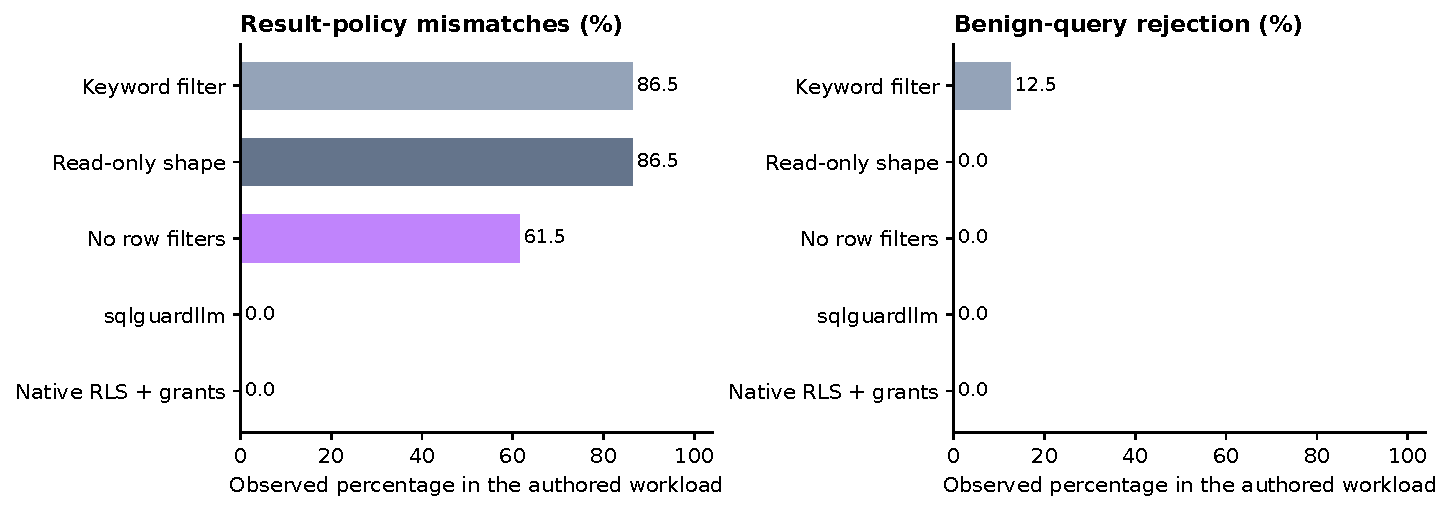
\includegraphics[width=\linewidth]{outcomes.pdf}
\caption{Descriptive outcome rates. The first four configurations pool
288 observations each across three runtimes; native RLS has 96 observations
in PostgreSQL/WASM. The benign-rejection denominator is 144 observations
for the first four methods and 48 for native RLS. These are correlated,
study-authored cases, not estimates of unseen attack prevalence.}
\label{fig:outcomes}
\end{figure}

Native RLS plus column grants matched the full guard on the tested
PostgreSQL/WASM workload: 72 authorized matches and 24 blocked forbidden
reads. This is evidence for complementarity and a sanity check on the oracle,
not evidence that application-layer rewriting improves on correctly configured
native access control. The shared target is authorized execution; portability
and agent-facing feedback are separate engineering considerations.

\subsection{Validation overhead and regression evidence}
Median warm validation times for the full guard were \SqliteMedian{} ms
for the SQLite dialect, \DuckdbMedian{} ms for DuckDB, and \PgliteMedian{}
ms for PostgreSQL. Corresponding p95 values were \SqliteTail{},
\DuckdbTail{}, and \PgliteTail{} ms. Figure~\ref{fig:latency} summarizes
these measurements. Because this stage runs in Python before database
execution, the labels identify the selected SQL dialect and the associated
execution run rather than database-server validation performance.

\begin{figure}[htbp]
\centering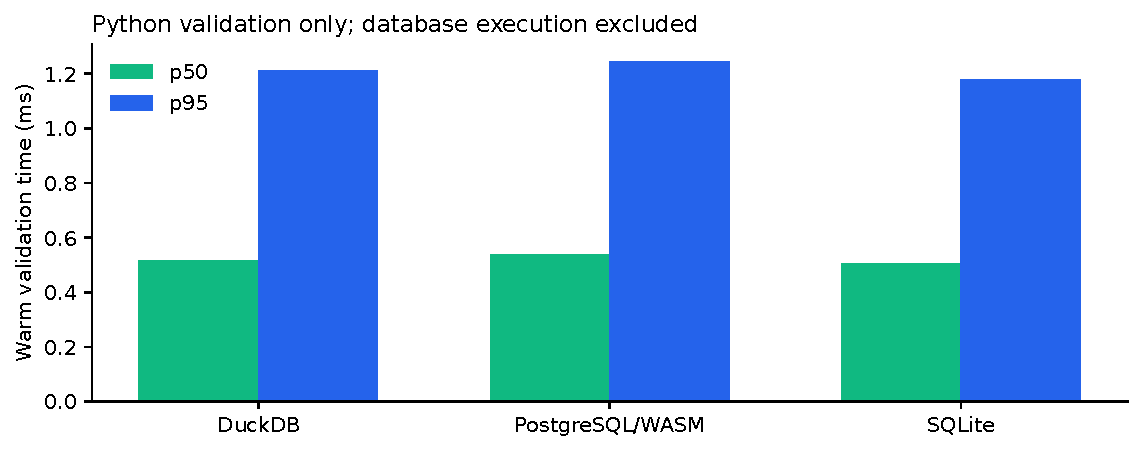
\includegraphics[width=.86\linewidth]{latency.pdf}
\caption{Measured warm full-guard validation times, excluding database
execution and policy compilation. All measurements come from the accompanying
raw per-call timing samples on one shared host.}
\label{fig:latency}
\end{figure}

Separately, \RegressionPassed{} existing development regression cases passed
their expected admission/rejection, violation-code, and specified output
fragment checks. They cover ten parser dialect labels: PostgreSQL, T-SQL,
Oracle, MySQL, SQLite, DuckDB, Snowflake, BigQuery, ClickHouse, and Trino.
This corpus is development evidence and must not be interpreted as real-engine
execution on ten database products. Its distribution is deliberately uneven,
and passing it establishes no statistical security guarantee.

\section{Related Work and Positioning}
Peng et al.\ \cite{peng2024security} investigate how text-to-SQL model
vulnerabilities can become software-security threats. SecureSQL
\cite{song2024securesql} evaluates sensitive-data leakage and attacks in
natural-language database interfaces. Its broad task and policy conditions
are not equivalent to this study's fixed, executable tenant policy; we do
not report results on SecureSQL or imply that its benchmark has been solved.
Fei et al.\ \cite{fei2026rbac} explicitly study text-to-SQL under role-based
access restrictions and motivate reporting utility separately from policy
compliance. Our execution oracle follows that separation in a smaller,
fully inspectable systems experiment.

Native row policies and column grants are mature database mechanisms
\cite{postgresrls}. SQLGlot supplies the parsing, expression representation,
and generation on which the library depends \cite{sqlglot}. The contribution
here is the particular open implementation and reproducible evaluation,
rather than a claim that AST validation or query rewriting is new. We do not
provide an exhaustive comparison with existing SQL-security libraries;
additional independent implementations and external workloads are important
next comparisons.

\section{Limitations and Threats to Validity}
\paragraph{Coverage and independence.}
The execution workload has 48 authored templates, two tenant contexts, a
small fixture, and three execution runtimes. Its authors knew the system
under evaluation, and no independent red-team or external test-set collection
was performed. We therefore avoid confidence intervals that would imply
randomly sampled, independent attack observations. The workload does not
cover all parser constructs, catalog access patterns, views, UDFs, engine
extensions, or complex schema-resolution cases.

\paragraph{Security scope.}
Zero observed mismatches is not a proof of safety for arbitrary SQL. The
library's correctness depends on parser and generator behavior and on a
correct, trusted policy. Masking, minimum aggregate group sizes, inference
across repeated queries, and cost protection require separate evaluation.
The study evaluates SQL presented at the execution boundary, not the rate
of prompt-injection success or natural-language answer correctness.

\paragraph{Execution and measurement.}
PGlite executes PostgreSQL compiled to WebAssembly; its behavior and resource
profile cannot substitute for a native server deployment study. No SQL Server,
MySQL, Oracle, or warehouse server was executed. Databases are tiny, so we
make no query-plan or database-overhead claim about derived-table rewriting.
The observation cap and bag comparison do not verify output ordering beyond
the explicit order needed to select capped rows. Warm validation timings
exclude compilation and use a fixed method order on one shared machine.

\paragraph{Baseline interpretation.}
The keyword and shape checks intentionally omit authorization functionality.
They illustrate failure modes, not competitive state-of-the-art defenses.
The row-filter ablation isolates one policy component. The correctly configured
native-RLS comparator performs equally on this workload and remains an
appropriate enforcement layer in deployments that support it.

\section{Conclusion}
\texttt{sqlguardllm} provides a deterministic interface for policy-driven
validation and rewriting of untrusted SQL. An execution study using
physically restricted reference databases observed correct authorized
results and forbidden-read rejection in 288 full-policy observations across
SQLite, DuckDB, and PostgreSQL/WASM. Removing row filters retained query-shape
checks while breaking result-level tenant compliance in many tested cases.
Native RLS and grants matched the full guard on the PostgreSQL/WASM workload.
The artifacts support independent reproduction and targeted extension;
broader workloads, independent adversarial evaluation, and native-server
measurements are required to assess generality.

\section*{Artifacts and Reproducibility}
Code and data are available at \url{https://github.com/jmmana/sqlguardllm},
under \texttt{research/}. The evaluated engine source is commit
\texttt{d73ad788434ea4e9f2601e2cc4fe41dd6877c38a}; raw metadata also records
a SHA-256 fingerprint of the engine's Python source and the workload.
The package is Apache-2.0 licensed. The study contains only synthetic data,
uses no model API calls, and includes per-case decisions, result rows,
individual timing samples, a versioned workload, and package/runtime versions.
Instructions distinguish the execution experiment from the regression corpus
and explain how to build this manuscript and regenerate figures and media.

\section*{Use of Generative AI Tools}
Generative AI tools assisted with drafting, evaluation-harness implementation,
and figure/media-generation code. The reported measurements were generated
by the included executable scripts rather than inferred from model output.
The author is responsible for final verification of all claims, references,
and released artifacts. This manuscript is provided for author review before
submission.

\begin{thebibliography}{9}
\bibitem{peng2024security}
Xutan Peng, Yipeng Zhang, Jingfeng Yang, and Mark Stevenson.
\newblock On the Security Vulnerabilities of Text-to-SQL Models.
\newblock arXiv:2211.15363, version 4, 2024.
\newblock \url{https://arxiv.org/abs/2211.15363}.

\bibitem{song2024securesql}
Yanqi Song, Ruiheng Liu, Shu Chen, Qianhao Ren, Yu Zhang, and Yongqi Yu.
\newblock SecureSQL: Evaluating Data Leakage of Large Language Models as
Natural Language Interfaces to Databases.
\newblock In \emph{Findings of EMNLP}, pages 5975--5990, 2024.
\newblock \url{https://doi.org/10.18653/v1/2024.findings-emnlp.346}.

\bibitem{fei2026rbac}
Yang Fei, Yangfan Jiang, Yin Yang, and Xiaokui Xiao.
\newblock Benchmarking Text-to-SQL under Role-Based Access Control.
\newblock arXiv:2607.22115, version 2, 2026.
\newblock \url{https://arxiv.org/abs/2607.22115}.

\bibitem{postgresrls}
PostgreSQL Global Development Group.
\newblock Row Security Policies. PostgreSQL documentation, 2026.
\newblock \url{https://www.postgresql.org/docs/19/ddl-rowsecurity.html}.

\bibitem{sqlglot}
Toby Mao and SQLGlot contributors.
\newblock SQLGlot: SQL Parser, Transpiler, Optimizer, and Engine.
\newblock Software, version 30.35.0, 2026.
\newblock \url{https://github.com/tobymao/sqlglot}.

\bibitem{pglite}
ElectricSQL and PGlite contributors.
\newblock PGlite: PostgreSQL in WebAssembly.
\newblock Software, version 0.6.0, 2026.
\newblock \url{https://pglite.dev/docs/}.
\end{thebibliography}

\appendix
\section{Reproduction Commands}
From the repository root, create an isolated environment so research database
drivers do not alter optional-dependency assumptions in the normal test suite:
\begin{lstlisting}[language=bash]
uv venv .venv-research
uv pip install --python .venv-research/bin/python \
  -r research/requirements.txt
npm ci --prefix research --ignore-scripts
.venv-research/bin/python research/evaluate.py
.venv-research/bin/python research/make_figures.py
cd research/paper
latexmk -pdf -interaction=nonstopmode main.tex
\end{lstlisting}
The paper's raw run used 50 timing rounds and five warm-ups. A smaller smoke
run may use \texttt{--engines sqlite --rounds 3 --warmup 1 --out /tmp/study}.
The native test suite is run in its separate locked development environment.
No credentials or externally hosted database are required for this experiment.

\section{Interpreting a Demo Result}
The README demonstrations are generated from \texttt{examples/readme\_demo.py}.
Their PostgreSQL-dialect checks return actual \texttt{CheckResult} fields;
only accepted portable reads execute on a synthetic SQLite fixture. For
tenant 7, the fixture has invoices $(1,7,250)$ and $(3,7,120)$ and another
tenant's invoice $(2,999,900)$. A tautological cross-tenant request returns
only $[(1,250),(3,120)]$ after rewriting. A write inside a CTE returns
\texttt{ok=false}, \texttt{sql=null}, and \texttt{write\_operation}; a private
email projection returns \texttt{hidden\_column}. The captioned videos and
GIFs are scripted visual explanations of these captured executions, not
recordings of a browser interface and not evidence for untested engines.
\end{document}
